\documentclass[border=10pt]{standalone}

\usepackage{tikz}
\usepackage{tikzsymbols}
\usetikzlibrary{calc,patterns,shapes.geometric}

\def\centerarc[#1](#2)(#3:#4:#5){\draw[#1] ($(#2)+({#5*cos(#3)},{#5*sin(#3)})$) arc (#3:#4:#5);}

\begin{document}
	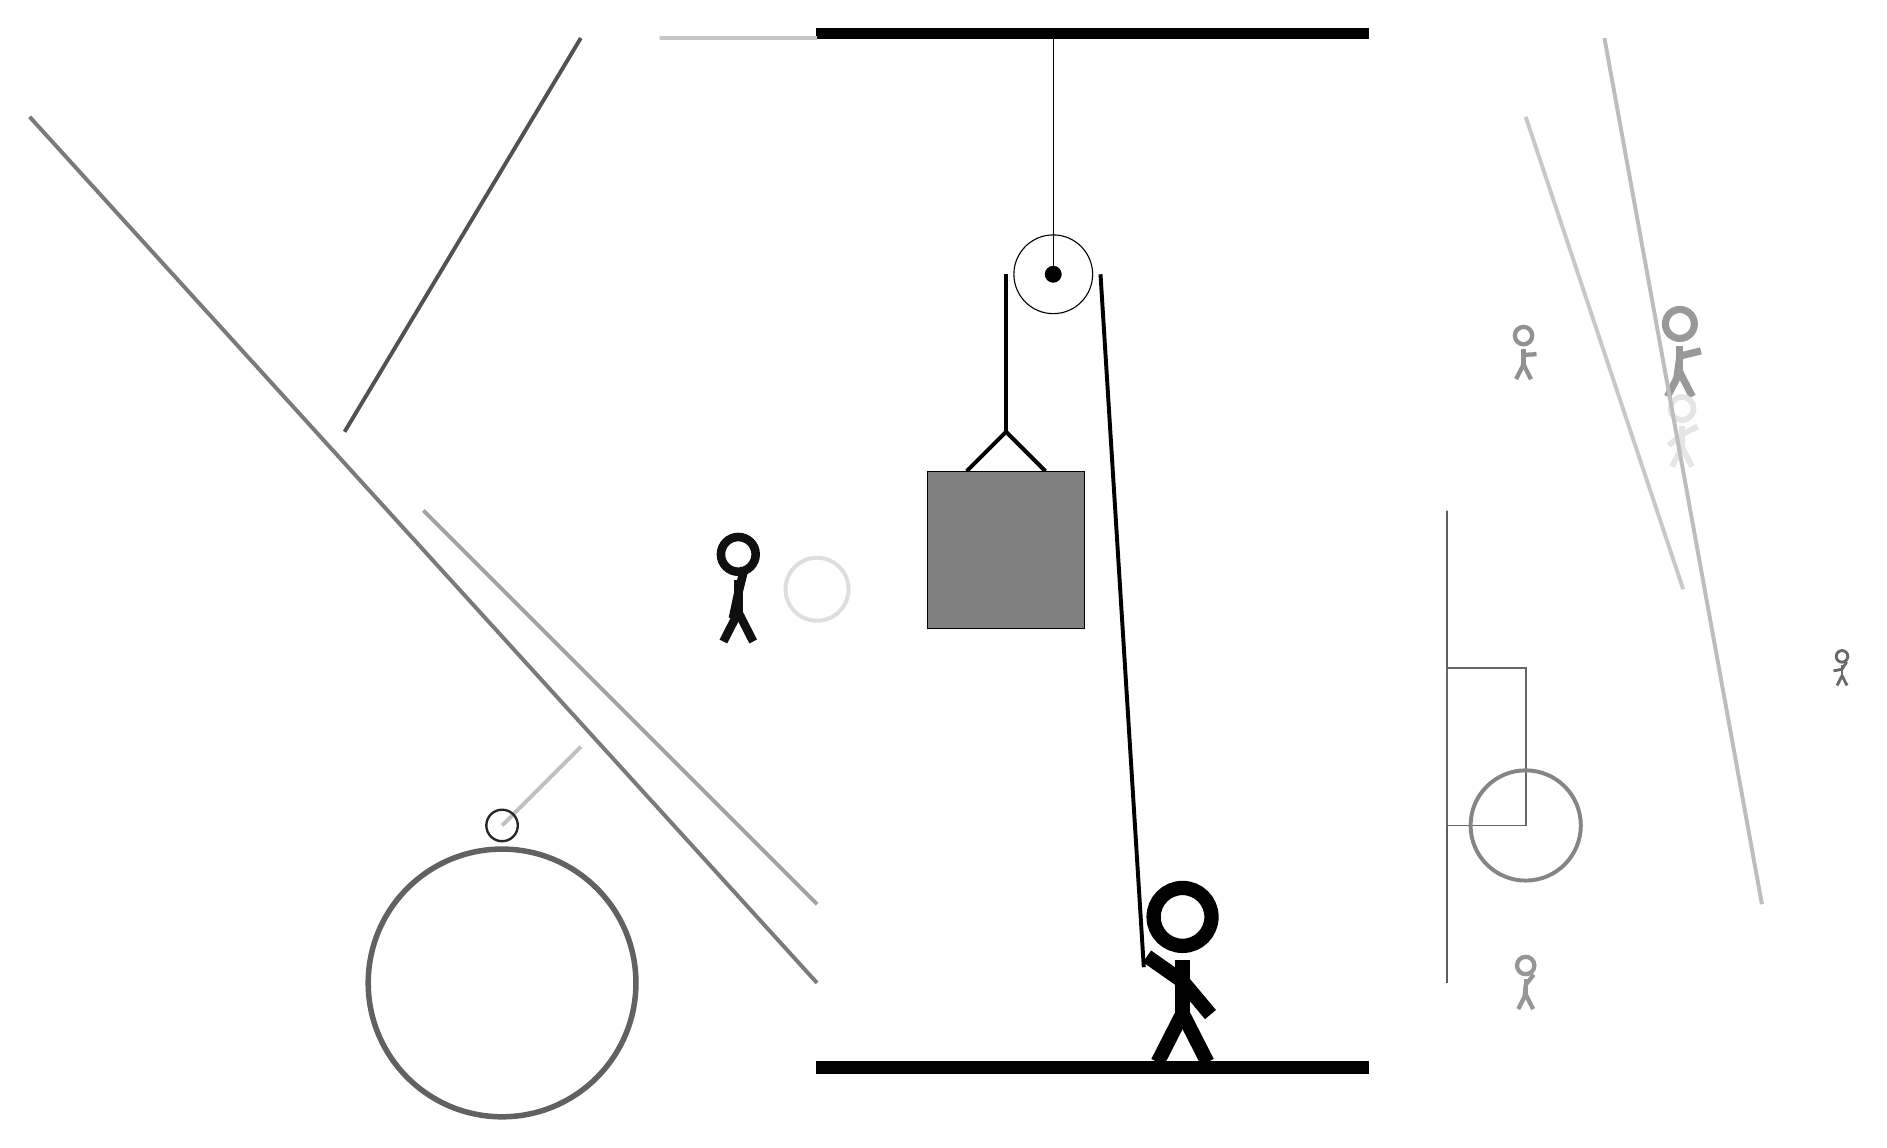
\begin{tikzpicture}
		%%%%% START %%%%%
		
		\draw[fill=black] (-2, 10) rectangle (5, 10.125);
		
		\draw (1, 7) circle (0.5);
		\draw[fill=black] (1, 7) circle (0.1);
		\draw (1, 10) -- (1, 7);
		
		\draw[line width=0.5mm] (-0.1, 4.5) -- (0.4, 5.0) -- (0.9, 4.5);
		\draw[fill=black!50] (-0.6, 4.5) rectangle (1.4, 2.5);
		
		\node[line width=0.4mm, color=black!40] at (9, 6) {\Strichmaxerl[5][82][14]};
		
		\draw[line width=0.5mm, color=black!68](-5, 10) -- (-8, 5);
		\node[line width=0.2mm, color=black!10] at (9, 5) {\Strichmaxerl[4][40][26]};
		\draw [line width=0.5mm, color=black!13](-2, 3) circle (0.4);
		\draw[line width=0.5mm, color=black!26](10, -1) -- (8, 10);
		\draw[line width=0.3mm, color=black!63] (6, 4) rectangle (6, -2);
		\draw[line width=0.2mm, color=black!60] (7, 0) rectangle (6, 2);
		\draw[line width=0.5mm, color=black!21](7, 9) -- (9, 3);
		\node[line width=0.2mm, color=black!41] at (7, -2) {\Strichmaxerl[3][85][52]};
		
		\node[line width=0.3mm, color=black!59] at (11, 2) {\Strichmaxerl[2][11][58]};
		\draw[line width=0.5mm, color=black!25](-6, 0) -- (-5, 1);
		\draw[line width=0.5mm, color=black!52](-2, -2) -- (-12, 9);
		\node[line width=0.2mm, color=black!94] at (-3, 3) {\Strichmaxerl[6][78][76]};
		\draw [line width=0.7mm, color=black!62](-6, -2) circle (1.7);
		\node[line width=0.2mm, color=black!43] at (7, 6) {\Strichmaxerl[3][87][3]};
		\draw [line width=0.5mm, color=black!48](7, 0) circle (0.7);
		\draw [line width=0.3mm, color=black!85](-6, 0) circle (0.2);
		
		\draw[line width=0.6mm, color=black!22] (-2, 10) rectangle (-4, 10);
		\draw[line width=0.5mm, color=black!36](-7, 4) -- (-2, -1);
		
		\draw[line width=0.5mm] (0.4, 7) -- (0.4, 5.0);
		\centerarc[line width=0.5mm](1, 7)(0:180:0.6);
		\draw[line width=0.5mm](1.6, 7) -- (2.15, -1.8);
		
		\node at (2.6, -1.9) {\Strichmaxerl[10][-35][-50]};
		
		\draw[fill=black] (-2, -3) rectangle (5, -3.15);
		
		%%%%% END %%%%%
	\end{tikzpicture}
\end{document}